\documentclass[11pt]{article}

\usepackage{report}

\usepackage{caption}

\usepackage[utf8]{inputenc} % allow utf-8 input
\usepackage[italian]{babel}
\usepackage[T1]{fontenc}    % use 8-bit T1 fonts
\usepackage[colorlinks=true, linkcolor=black, citecolor=blue, urlcolor=blue]{hyperref}       % hyperlinks
\usepackage{url}            % simple URL typesetting
\usepackage{booktabs}       % professional-quality tables
\usepackage{amsfonts}       % blackboard math symbols
\usepackage{nicefrac}       % compact symbols for 1/2, etc.
\usepackage{microtype}      % microtypography
\usepackage{lipsum}		% Can be removed after putting your text content
\usepackage{graphicx}
\usepackage{natbib}
\usepackage{doi}
\setcitestyle{aysep={,}}

% tree structure
\usepackage{forest}
%%%%%%%%%


%%%%%%%%%%%%%% CODE

\usepackage{listings}
\usepackage{color} %red, green, blue, yellow, cyan, magenta, black, white
\definecolor{mygreen}{RGB}{28,172,0} % color values Red, Green, Blue
\definecolor{mylilas}{RGB}{170,55,241}

\lstset{language=Matlab,%
    %basicstyle=\color{red},
    breaklines=true,%
    morekeywords={matlab2tikz},
    keywordstyle=\color{blue},%
    morekeywords=[2]{1}, keywordstyle=[2]{\color{black}},
    identifierstyle=\color{black},%
    stringstyle=\color{mylilas},
    commentstyle=\color{mygreen},%
    showstringspaces=false,%without this there will be a symbol in the places where there is a space
    numbers=left,%
    numberstyle={\tiny \color{black}},% size of the numbers
    numbersep=9pt, % this defines how far the numbers are from the text
    emph=[1]{for,end,break},emphstyle=[1]\color{red}, %some words to emphasise
    %emph=[2]{word1,word2}, emphstyle=[2]{style},    
}

%----------------------------------------------------------------------------------------
%	PYTHON CODE THEMPLATE
%----------------------------------------------------------------------------------------
\usepackage{listings}
\usepackage{xcolor}

\definecolor{codegreen}{rgb}{0,0.6,0}
\definecolor{codegray}{rgb}{0.5,0.5,0.5}
\definecolor{codepurple}{rgb}{0.58,0,0.82}
\definecolor{backcolour}{rgb}{0.95,0.95,0.92}

\lstset{language=Matlab,%
     % backgroundcolor=\color{backcolour},
    commentstyle=\color{codegreen},
    keywordstyle=\color{magenta},
    numberstyle=\tiny\color{codegray},
    stringstyle=\color{codepurple},
    basicstyle=\ttfamily\footnotesize,
    breakatwhitespace=false,
    breaklines=true,
    captionpos=b,
    keepspaces=true,
    numbers=left,
    numbersep=5pt,
    showspaces=false,
    showstringspaces=false,
    showtabs=false,
    aboveskip=6mm,
    belowskip=6mm,
    tabsize=2   
}
%%%%%%%%%%%%%%

\title{Cholesky Analysis}

\author{
  \Large\textbf{Mario Avolio}\\
  \texttt{800995}
  \and
  \Large\textbf{Simone Benitozzi}\\
  \texttt{889407}
}

% Uncomment to remove the date
\date{\today}

% Uncomment to override  the `A preprint' in the header
\renewcommand{\headeright}{Cholesky Analysis - Metodi del calcolo Scientifico}
\renewcommand{\undertitle}{Metodi del calcolo Scientifico}
\renewcommand{\shorttitle}{}

%%% Add PDF metadata to help others organize their library
%%% Once the PDF is generated, you can check the metadata with
%%% $ pdfinfo template.pdf
% \hypersetup{
% pdftitle={A template for the arxiv style},
% pdfsubject={q-bio.NC, q-bio.QM},
% pdfauthor={David S.~Hippocampus, Elias D.~Striatum},
% pdfkeywords={First keyword, Second keyword, More},
% }

\begin{document}
\maketitle

\newpage
\tableofcontents
\thispagestyle{empty}

\newpage
\thispagestyle{empty}


\newpage
\setcounter{page}{1}
\section{Introduzione}
TODO: Introduzione






\section{Descrizione del dominio di riferimento e obiettivi dell’elaborato} % cholesky 

\section{Scelte di design} % presentiamo il codice
\subsection{Matlab}
TODO: Come ho fatto il matlab?
\subsection{Python}
Per gestire al meglio la giusta separazione tra gli elementi del progetto si è deciso di sfruttare un particolare pattern strutturale definito dallo schema sottostante. Il modello, cattura il comportamento dell'applicazione in termini di dominio del problema e gestisce direttamente i dati, la logica e le regole del progetto. 


\begin{forest}
  for tree={
    font=\ttfamily,
    grow'=0,
    child anchor=west,
    parent anchor=south,
    anchor=west,
    calign=first,
    edge path={
      \noexpand\path [draw, \forestoption{edge}]
      (!u.south west) +(7.5pt,0) |- node[fill,inner sep=1.25pt] {} (.child anchor)\forestoption{edge label};
    },
    before typesetting nodes={
      if n=1
        {insert before={[,phantom]}}
        {}
    },
    fit=band,
    before computing xy={l=15pt},
  }
[Customer Personality Analysis Project
  [ML-Porject.Rproj]
  [Data
    [marketing\_campaign.csv]
  ]
  [DOC
    [Presentation
    [...]]
    [Report
    [...]]
  ]
  [Script
  [D-TREE.R]
  [DescriptionOfData.R]
  [EDA.R]
  [K-MEANS.R]
  [PCA.R]
  [D-TREE-Model Evaluation.R]
  [Functions
  [Functions.R]]
  ]
  [Output
  [Plots
  [...]]
  [Data
  [...]]]
  [Other
  [...]]
  [README.MD]
]
\end{forest}\\

\section{Descrizione dei Dati} % matrici

%######################################################################%
%||                                                                  %||
%||                                                                  %||
%||                            NEW MATRIX                            %||
%||                                                                  %||
%||                                                                  %||
%######################################################################%

\subsection{Flan-1565}
\begin{table}[h!]
	\begin{minipage}{0.5\linewidth}
		\caption{Flan-1565 Information}
		\label{table:Flan-1565}
		\centering
        \begin{tabular}{ll}
\midrule
                       Name &              Flan\_1565 \\
                      Group &                  Janna \\
                  Matrix ID &                   2544 \\
                   Num Rows &                1564794 \\
                   Num Cols &                1564794 \\
                   Nonzeros &              114165372 \\
            Pattern Entries &              117406044 \\
                       Kind &     Structural Problem \\
                  Symmetric &                    Yes \\
                       Date &                   2011 \\
                     Author & C. Janna, M. Ferronato \\
                     Editor &               T. Davis \\
            Structural Rank &                1564794 \\
       Structural Rank Full &                   true \\
          Num Dmperm Blocks &                      1 \\
Strongly Connect Components &                      1 \\
         Num Explicit Zeros &                3240672 \\
           Pattern Symmetry &                   100\% \\
           Numeric Symmetry &                   100\% \\
         Cholesky Candidate &                    yes \\
          Positive Definite &                    yes \\
                       Type &                   real \\
\bottomrule
\end{tabular}

	\end{minipage}\hfill
	\begin{minipage}{0.45\linewidth}
		\centering
		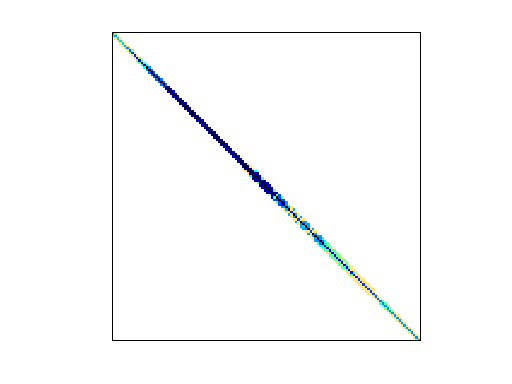
\includegraphics[width=1\textwidth]{figs/Flan_1565.png}
		\captionof{figure}{Flan-1565}
		\label{fig:Flan-1565}
	\end{minipage}
\end{table}

%######################################################################%
%||                                                                  %||
%||                                                                  %||
%||                            NEW MATRIX                            %||
%||                                                                  %||
%||                                                                  %||
%######################################################################%

\subsection{StocF-1465}
\begin{table}[h!]
	\begin{minipage}{0.5\linewidth}
		\caption{StocF-1465 Information}
		\label{table:StocF-1465}
		\centering
        \begin{tabular}{ll}
\midrule
                       Name &                           StocF-1465 \\
                      Group &                                Janna \\
                  Matrix ID &                                 2547 \\
                   Num Rows &                              1465137 \\
                   Num Cols &                              1465137 \\
                   Nonzeros &                             21005389 \\
            Pattern Entries &                             21005389 \\
                       Kind & CFDP \\
                  Symmetric &                                  Yes \\
                       Date &                                 2011 \\
                     Author &               C. Janna, M. Ferronato \\
                     Editor &                             T. Davis \\
            Structural Rank &                              1465137 \\
       Structural Rank Full &                                 true \\
          Num Dmperm Blocks &                                29105 \\
Strongly Connect Components &                                29105 \\
         Num Explicit Zeros &                                    0 \\
           Pattern Symmetry &                                 100\% \\
           Numeric Symmetry &                                 100\% \\
         Cholesky Candidate &                                  yes \\
          Positive Definite &                                  yes \\
                       Type &                                 real \\
\bottomrule
\end{tabular}

	\end{minipage}\hfill
	\begin{minipage}{0.45\linewidth}
		\centering
		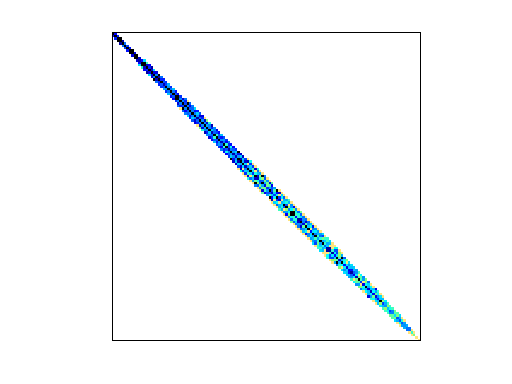
\includegraphics[width=1\textwidth]{figs/StocF-1465.png}
		\captionof{figure}{StocF-1465}
		\label{fig:StocF-1465}
	\end{minipage}
\end{table}


%######################################################################%
%||                                                                  %||
%||                                                                  %||
%||                            NEW MATRIX                            %||
%||                                                                  %||
%||                                                                  %||
%######################################################################%

\subsection{cfd2}
\begin{table}[h!]
	\begin{minipage}{0.5\linewidth}
		\caption{cfd2 Information}
		\label{table:cfd2}
		\centering
        \begin{tabular}{ll}
\midrule
                       Name &                                 cfd2 \\
                      Group &                             Rothberg \\
                  Matrix ID &                                  805 \\
                   Num Rows &                               123440 \\
                   Num Cols &                               123440 \\
                   Nonzeros &                              3085406 \\
            Pattern Entries &                              3087898 \\
                       Kind & CFDP \\
                  Symmetric &                                  Yes \\
                       Date &                                 1997 \\
                     Author &                          E. Rothberg \\
                     Editor &                             T. Davis \\
            Structural Rank &                               123440 \\
       Structural Rank Full &                                 true \\
          Num Dmperm Blocks &                                    1 \\
Strongly Connect Components &                                    1 \\
         Num Explicit Zeros &                                 2492 \\
           Pattern Symmetry &                                 100\% \\
           Numeric Symmetry &                                 100\% \\
         Cholesky Candidate &                                  yes \\
          Positive Definite &                                  yes \\
                       Type &                                 real \\
\bottomrule
\end{tabular}

	\end{minipage}\hfill
	\begin{minipage}{0.45\linewidth}
		\centering
		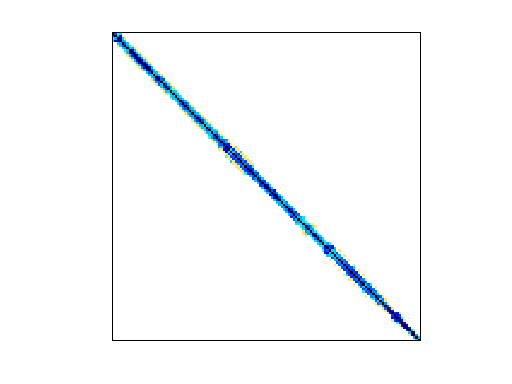
\includegraphics[width=1\textwidth]{figs/cfd2.png}
		\captionof{figure}{cfd2}
		\label{fig:cfd2}
	\end{minipage}
\end{table}


%######################################################################%
%||                                                                  %||
%||                                                                  %||
%||                            NEW MATRIX                            %||
%||                                                                  %||
%||                                                                  %||
%######################################################################%
\subsection{cfd1}
\begin{table}[h!]
	\begin{minipage}{0.5\linewidth}
		\caption{cdf1 Information}
		\label{table:cdf1}
		\centering
        \begin{tabular}{ll}
\midrule
                       Name &                                 cfd1 \\
                      Group &                             Rothberg \\
                  Matrix ID &                                  804 \\
                   Num Rows &                                70656 \\
                   Num Cols &                                70656 \\
                   Nonzeros &                              1825580 \\
            Pattern Entries &                              1828364 \\
                       Kind & CFDP \\
                  Symmetric &                                  Yes \\
                       Date &                                 1997 \\
                     Author &                          E. Rothberg \\
                     Editor &                             T. Davis \\
            Structural Rank &                                70656 \\
       Structural Rank Full &                                 true \\
          Num Dmperm Blocks &                                    1 \\
Strongly Connect Components &                                    1 \\
         Num Explicit Zeros &                                 2784 \\
           Pattern Symmetry &                                 100\% \\
           Numeric Symmetry &                                 100\% \\
         Cholesky Candidate &                                  yes \\
          Positive Definite &                                  yes \\
                       Type &                                 real \\
\bottomrule
\end{tabular}

	\end{minipage}\hfill
	\begin{minipage}{0.45\linewidth}
		\centering
		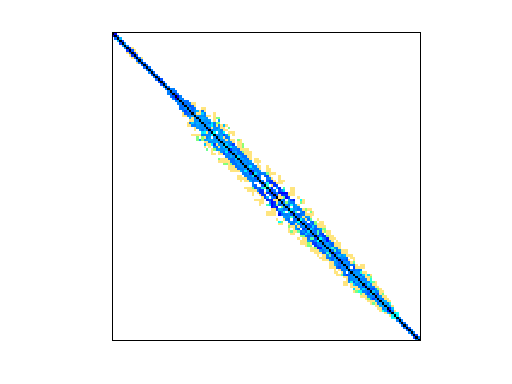
\includegraphics[width=1\textwidth]{figs/cfd1.png}
		\captionof{figure}{cdf1}
		\label{fig:cdf1}
	\end{minipage}
\end{table}



%######################################################################%
%||                                                                  %||
%||                                                                  %||
%||                            NEW MATRIX                            %||
%||                                                                  %||
%||                                                                  %||
%######################################################################%
\subsection{G3-circuit}
\begin{table}[h!]
	\begin{minipage}{0.5\linewidth}
		\caption{G3-circuit Information}
		\label{table:cdf1}
		\centering
        \begin{tabular}{ll}
\midrule
                       Name &                 G3\_circuit \\
                      Group &                        AMD \\
                  Matrix ID &                       1421 \\
                   Num Rows &                    1585478 \\
                   Num Cols &                    1585478 \\
                   Nonzeros &                    7660826 \\
            Pattern Entries &                    7660826 \\
                       Kind & Circuit Simulation Problem \\
                  Symmetric &                        Yes \\
                       Date &                       2006 \\
                     Author &                 U. Okuyucu \\
                     Editor &                   T. Davis \\
            Structural Rank &                    1585478 \\
       Structural Rank Full &                       true \\
          Num Dmperm Blocks &                          1 \\
Strongly Connect Components &                          1 \\
         Num Explicit Zeros &                          0 \\
           Pattern Symmetry &                       100\% \\
           Numeric Symmetry &                       100\% \\
         Cholesky Candidate &                        yes \\
          Positive Definite &                        yes \\
                       Type &                       real \\
\bottomrule
\end{tabular}

	\end{minipage}\hfill
	\begin{minipage}{0.45\linewidth}
		\centering
		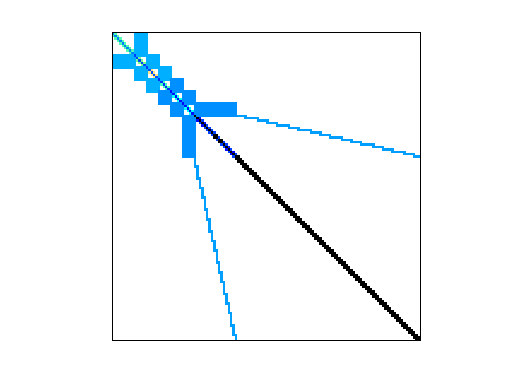
\includegraphics[width=1\textwidth]{figs/G3_circuit.png}
		\captionof{figure}{G3-circuit}
		\label{fig:G3-circuit}
	\end{minipage}
\end{table}



%######################################################################%
%||                                                                  %||
%||                                                                  %||
%||                            NEW MATRIX                            %||
%||                                                                  %||
%||                                                                  %||
%######################################################################%
\subsection{Parabolic Fem}
\begin{table}[h!]
	\begin{minipage}{0.5\linewidth}
		\caption{Parabolic Fem Information}
		\label{table:Parabolic Fem}
		\centering
        \begin{tabular}{ll}
\midrule
                       Name &                        parabolic\_fem \\
                      Group &                             Wissgott \\
                  Matrix ID &                                 1853 \\
                   Num Rows &                               525825 \\
                   Num Cols &                               525825 \\
                   Nonzeros &                              3674625 \\
            Pattern Entries &                              3674625 \\
                       Kind & CFDP \\
                  Symmetric &                                  Yes \\
                       Date &                                 2007 \\
                     Author &                          P. Wissgott \\
                     Editor &                             T. Davis \\
            Structural Rank &                               525825 \\
       Structural Rank Full &                                 true \\
          Num Dmperm Blocks &                                    1 \\
Strongly Connect Components &                                    1 \\
         Num Explicit Zeros &                                    0 \\
           Pattern Symmetry &                                 100\% \\
           Numeric Symmetry &                                 100\% \\
         Cholesky Candidate &                                  yes \\
          Positive Definite &                                  yes \\
                       Type &                                 real \\
\bottomrule
\end{tabular}

	\end{minipage}\hfill
	\begin{minipage}{0.45\linewidth}
		\centering
		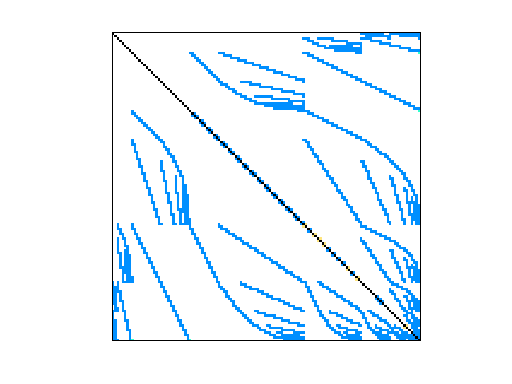
\includegraphics[width=1\textwidth]{figs/parabolic_fem.png}
		\captionof{figure}{Parabolic Fem}
		\label{fig:Parabolic Fem}
	\end{minipage}
\end{table}



%######################################################################%
%||                                                                  %||
%||                                                                  %||
%||                            NEW MATRIX                            %||
%||                                                                  %||
%||                                                                  %||
%######################################################################%
\subsection{apache2}
\begin{table}[h!]
	\begin{minipage}{0.5\linewidth}
		\caption{apache2 Information}
		\label{table:apache2}
		\centering
        \begin{tabular}{ll}
\midrule
                       Name &                   apache2 \\
                      Group &                 GHS\_psdef \\
                  Matrix ID &                      1423 \\
                   Num Rows &                    715176 \\
                   Num Cols &                    715176 \\
                   Nonzeros &                   4817870 \\
            Pattern Entries &                   4817870 \\
                       Kind &        Structural Problem \\
                  Symmetric &                       Yes \\
                       Date &                      2006 \\
                     Author &                       NaN \\
                     Editor & N. Gould, Y. Hu, J. Scott \\
            Structural Rank &                    715176 \\
       Structural Rank Full &                      true \\
          Num Dmperm Blocks &                         1 \\
Strongly Connect Components &                         1 \\
         Num Explicit Zeros &                         0 \\
           Pattern Symmetry &                      100\% \\
           Numeric Symmetry &                      100\% \\
         Cholesky Candidate &                       yes \\
          Positive Definite &                       yes \\
                       Type &                      real \\
\bottomrule
\end{tabular}

	\end{minipage}\hfill
	\begin{minipage}{0.45\linewidth}
		\centering
		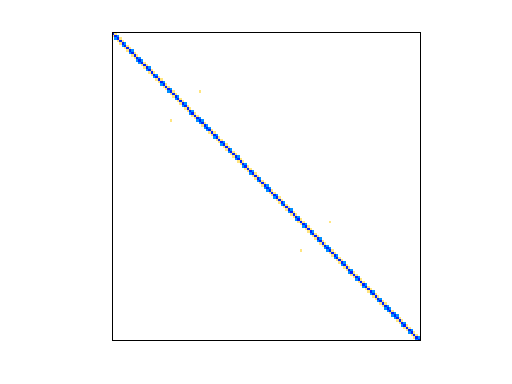
\includegraphics[width=1\textwidth]{figs/apache2.png}
		\captionof{figure}{apache2}
		\label{fig:apache2}
	\end{minipage}
\end{table}



%######################################################################%
%||                                                                  %||
%||                                                                  %||
%||                            NEW MATRIX                            %||
%||                                                                  %||
%||                                                                  %||
%######################################################################%
\subsection{shallow water1}
\begin{table}[h!]
	\begin{minipage}{0.5\linewidth}
		\caption{shallow water1 Information}
		\label{table:shallow water1}
		\centering
        \begin{tabular}{ll}
\midrule
                       Name &                       shallow\_water1 \\
                      Group &                            MaxPlanck \\
                  Matrix ID &                                 2261 \\
                   Num Rows &                                81920 \\
                   Num Cols &                                81920 \\
                   Nonzeros &                               327680 \\
            Pattern Entries &                               327680 \\
                       Kind & CFDP \\
                  Symmetric &                                  Yes \\
                       Date &                                 2009 \\
                     Author &               K. Leppkes, U. Naumann \\
                     Editor &                             T. Davis \\
            Structural Rank &                                81920 \\
       Structural Rank Full &                                 true \\
          Num Dmperm Blocks &                                    1 \\
Strongly Connect Components &                                    1 \\
         Num Explicit Zeros &                                    0 \\
           Pattern Symmetry &                                 100\% \\
           Numeric Symmetry &                                 100\% \\
         Cholesky Candidate &                                  yes \\
          Positive Definite &                                  yes \\
                       Type &                                 real \\
\bottomrule
\end{tabular}

	\end{minipage}\hfill
	\begin{minipage}{0.45\linewidth}
		\centering
		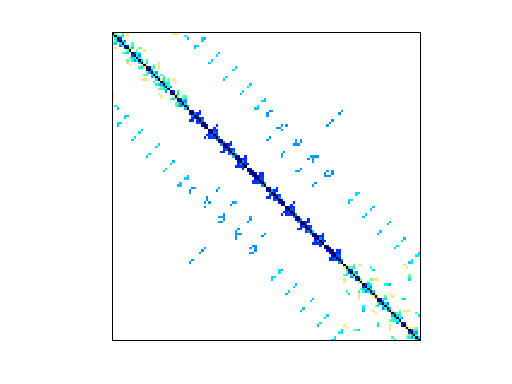
\includegraphics[width=1\textwidth]{figs/shallow_water1.png}
		\captionof{figure}{shallow water1}
		\label{fig:shallow water1}
	\end{minipage}
\end{table}




%######################################################################%
%||                                                                  %||
%||                                                                  %||
%||                            NEW MATRIX                            %||
%||                                                                  %||
%||                                                                  %||
%######################################################################%
\subsection{ex15}
\begin{table}[h!]
	\begin{minipage}{0.5\linewidth}
		\caption{ex15 Information}
		\label{table:ex15}
		\centering
        \begin{tabular}{ll}
\midrule
                       Name &                                 ex15 \\
                      Group &                                FIDAP \\
                  Matrix ID &                                  413 \\
                   Num Rows &                                 6867 \\
                   Num Cols &                                 6867 \\
                   Nonzeros &                                98671 \\
            Pattern Entries &                                98671 \\
                       Kind & CFDP \\
                  Symmetric &                                  Yes \\
                       Date &                                 1994 \\
                     Author &                   A. Baggag, Y. Saad \\
                     Editor &                   A. Baggag, Y. Saad \\
            Structural Rank &                                 6867 \\
       Structural Rank Full &                                 true \\
          Num Dmperm Blocks &                                    2 \\
Strongly Connect Components &                                    2 \\
         Num Explicit Zeros &                                    0 \\
           Pattern Symmetry &                                 100\% \\
           Numeric Symmetry &                                 100\% \\
         Cholesky Candidate &                                  yes \\
          Positive Definite &                                  yes \\
                       Type &                                 real \\
\bottomrule
\end{tabular}

	\end{minipage}\hfill
	\begin{minipage}{0.45\linewidth}
		\centering
		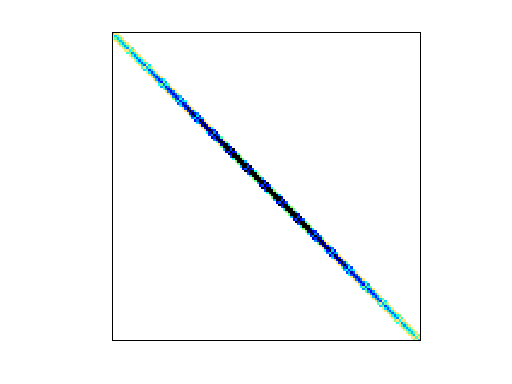
\includegraphics[width=1\textwidth]{figs/ex15.png}
		\captionof{figure}{ex15}
		\label{fig:ex15}
	\end{minipage}
\end{table}


\section{Risulti Sperimentali}
\subsection{Flan-1565}
\paragraph{Windows and Python}
ciao
\paragraph{Windows and Matlab}

\paragraph{Linux and Python}
\paragraph{Linux and Matlab}
% qual è stata la scelta migliore?

\subsection{StocF-1465}
\subsection{cfd2}
\subsection{cfd1}
\subsection{G3-circuit}
\subsection{parabolic fem} 
\subsection{apache2}
\subsection{shallow water1}
\subsection{ex15}


\section*{Conclusioni}




% BIBLIOGRAPHY
\bibliographystyle{unsrtnat}
\bibliography{references}  %%% Uncomment this line and comment out the ``thebibliography'' section below to use the external .bib file (using bibtex) .


%%% Uncomment this section and comment out the \bibliography{references} line above to use inline references.
% \begin{thebibliography}{1}

% 	\bibitem{kour2014real}
% 	George Kour and Raid Saabne.
% 	\newblock Real-time segmentation of on-line handwritten arabic script.
% 	\newblock In {\em Frontiers in Handwriting Recognition (ICFHR), 2014 14th
% 			International Conference on}, pages 417--422. IEEE, 2014.

% 	\bibitem{kour2014fast}
% 	George Kour and Raid Saabne.
% 	\newblock Fast classification of handwritten on-line arabic characters.
% 	\newblock In {\em Soft Computing and Pattern Recognition (SoCPaR), 2014 6th
% 			International Conference of}, pages 312--318. IEEE, 2014.

% 	\bibitem{hadash2018estimate}
% 	Guy Hadash, Einat Kermany, Boaz Carmeli, Ofer Lavi, George Kour, and Alon
% 	Jacovi.
% 	\newblock Estimate and replace: A novel approach to integrating deep neural
% 	networks with existing applications.
% 	\newblock {\em arXiv preprint arXiv:1804.09028}, 2018.

% \end{thebibliography}


\end{document}
